\chapter{State of the Art}

This project aims to create a serious game based on a robot in a remote laboratory. Moreover, it
aims to create a complete visual programming experience to teach the basics of programming. Thus,
in this state of the art, I will cover the three main topics that the project uses as a base and I
will deepen into them.

\section{Remote laboratories}

As we have seen in previous sections, remote laboratories can be really helpful in teaching main
concepts about science and technology. In this section I will analyse which is the current status of
remote experimentation around the world and I will show examples of how do remote laboratories work
in various scenarios.

\subsection{Global Online Laboratory Consortium}

The Global Online Laboratory Consortium or \textit{GOLC} is an organization that focuses on
the promotion of the development of remote laboratories for educational use. They commonly promote
remote laboratories through conferences~\cite{golc1st}. They also support and encourage the sharing
of these laboratories between institutions.

For promoting laboratories, they created an award (Figure~\ref{fig:golc_award}) for remote
experimentation and another one for simulated experimentation.

\begin{figure}[!htbp]
	\centering
	
\includegraphics[width=.4\textwidth]{fig/golc_award}
	\caption{GOLC Online Laboratory Award 2015}\label{fig:golc_award}
\end{figure}

\subsection{WebLab-Deusto}

WebLab-Deusto is a remote laboratory located at the University of Deusto, Bilbao. There are multiple
types of laboratories there, and all is being controlled by a software they developed, called
WebLab. Moreover, Pablo Orduña, one of it's main researches developed a complete federation model
to be able to share laboratories across the world~\cite{porduna_phd}.

% TODO insert picture from WebLab

In Weblab-Deusto they created one of the most used remote laboratories in electronics teaching. It
is called VISIR~\cite{visir}, and it recreates circuits made visually by students in real hardware
so that students can take real measurements.

\begin{figure}[!htbp]
	\centering
	
\includegraphics[width=.4\textwidth]{fig/weblab}
	\caption{WebLab-Deusto logo.}
\end{figure}

\subsection{iLab Project at MIT}

The Massachusetts Institute of Technology has its own remote laboratory platform called iLab. They
have many remote laboratories where they experiment with Dynamic Signal Analyzers, Heat Exchangers
and even with Polymer Crystallization. It has even inspired some big projects using this technology
such as an on-line repository to locate remote laboratories~\cite{ilabs_multi}.

\begin{figure}[!htbp]
	\centering
	
\includegraphics[width=.4\textwidth]{fig/icampus}
	\caption{iCampus logo, project at MIT where iLabs have been created.}
\end{figure}

\subsection{Robotic remote experiments}

Some of the laboratories listed before have currently implementations of robotic experiments in
as a teaching material in some areas. In WebLab-Deusto, for example, they have what they call
WebLab-Bot. This robot is based on Azkar-Bot robot and it is used for electronic students to learn
how to program it. They have simple demonstrations that follow a black line or respond to simple
commands.

% TODO img WebLab-Bot

Moreover, in The Labshare Institute, they have a robot called iRobot, that teaches how to deal with
accuracy of sensors and localization and mapping. Finally, the robot that will be used in this
project is called Romie. It is located in WebLab-Deusto and it has the needed functionality for this
project: it is capable of following a line, it detects walls and it detects intersections.

% TODO img Romie

\subsection{Simulations}

Even if the project will not be based on simulated robotics but in real robots, currently many
many projects use simulations to bring some of the experience to users. A simulation is usually
less costly than a remote laboratory, since not much hardware is required. On the other hand,
students will not be using real tools and experimentation environments, so the experience of using
them will not be as complete as in a remote laboratory.

Nevertheless, some prefer creating hybrid laboratories~\cite{hybrid_labs}. In these cases, the
laboratories add a simulation layer over the real laboratory. This way, the user still uses a real
laboratory, with the benefits of knowing how to use the laboratory and doing real experimentation,
and it also gives the user some more benefit by simulating extra conditions that could be expensive
to create in a real laboratory.

\section{Serious Games}

\section{Visual Programming}

Visual programming is a way of programming that instead of using real code in a real programming
language uses a visual interface to create programs and then translate them to a well known
language. This way, people that are not yet used to programming languages, interfaces such as IDEs
or code execution, and do not understand the basis of programming can start learning by using a
simple visual environment~\cite{visual_programming}.

\subsection{Scratch}

Scratch is one of the most known visual programming tools~\cite{scratch}. It is in itself an IDE,
made by the MIT to help to teach programming to inexperienced users. It teaches the basic concepts
of algorithms and it gives an enough powerful tool so that users can enjoy using it. It's main
concept is to join basic programming blocks so that functionality is created.

Moreover, they have created a complete collaboration platform where all the users of Scratch can
share their creations and check out the ones that others have made. That way, users can learn more
by looking at code created by others.

\subsection{Blockly}

Blockly, unlike Scratch, is not a visual programming IDE, but a visual programming library to create
visual programming editors and IDEs. It has the same basis as Scratch, so it contains basic
programming blocks to build applications by joining them (Figure~\ref{fig:blockly}), and it also
gives developers the option to create their own blocks with a simple API. It was created by Google
and it's source is now available in GitHub.

\begin{figure}[!htbp]
	\centering
	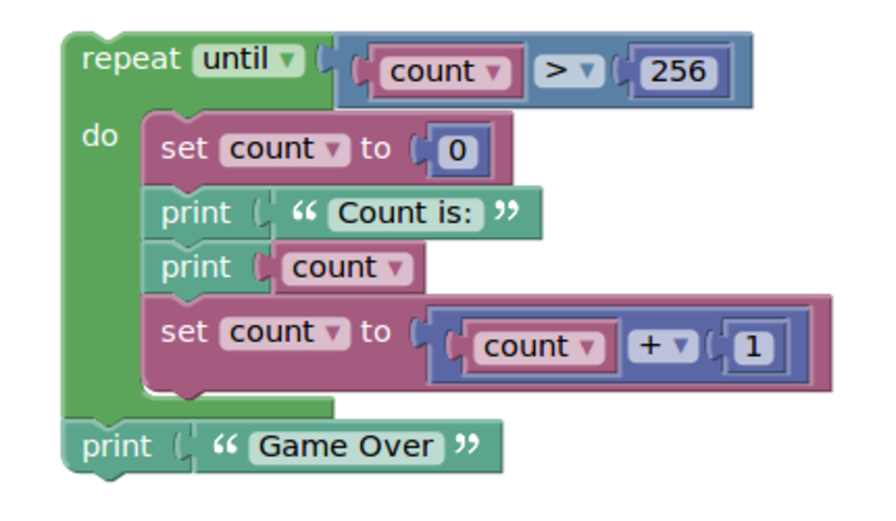
\includegraphics[width=.5\textwidth]{fig/blockly}
	\caption{Simple program example created in Google's Blockly.}\label{fig:blockly}
\end{figure}

Blockly enables developers to create their own programming environments for their projects, so they
can adapt Blockly itself to their needs, and thus, making it possible for them to even create
complete IDEs for their projects based on visual programming.


